% Options for packages loaded elsewhere
% Options for packages loaded elsewhere
\PassOptionsToPackage{unicode}{hyperref}
\PassOptionsToPackage{hyphens}{url}
\PassOptionsToPackage{dvipsnames,svgnames,x11names}{xcolor}
%
\documentclass[
  12pt,
  letterpaper,
  DIV=11,
  numbers=noendperiod]{scrartcl}
\usepackage{xcolor}
\usepackage[margin=1in]{geometry}
\usepackage{amsmath,amssymb}
\setcounter{secnumdepth}{5}
\usepackage{iftex}
\ifPDFTeX
  \usepackage[T1]{fontenc}
  \usepackage[utf8]{inputenc}
  \usepackage{textcomp} % provide euro and other symbols
\else % if luatex or xetex
  \usepackage{unicode-math} % this also loads fontspec
  \defaultfontfeatures{Scale=MatchLowercase}
  \defaultfontfeatures[\rmfamily]{Ligatures=TeX,Scale=1}
\fi
\usepackage{lmodern}
\ifPDFTeX\else
  % xetex/luatex font selection
\fi
% Use upquote if available, for straight quotes in verbatim environments
\IfFileExists{upquote.sty}{\usepackage{upquote}}{}
\IfFileExists{microtype.sty}{% use microtype if available
  \usepackage[]{microtype}
  \UseMicrotypeSet[protrusion]{basicmath} % disable protrusion for tt fonts
}{}
\makeatletter
\@ifundefined{KOMAClassName}{% if non-KOMA class
  \IfFileExists{parskip.sty}{%
    \usepackage{parskip}
  }{% else
    \setlength{\parindent}{0pt}
    \setlength{\parskip}{6pt plus 2pt minus 1pt}}
}{% if KOMA class
  \KOMAoptions{parskip=half}}
\makeatother
% Make \paragraph and \subparagraph free-standing
\makeatletter
\ifx\paragraph\undefined\else
  \let\oldparagraph\paragraph
  \renewcommand{\paragraph}{
    \@ifstar
      \xxxParagraphStar
      \xxxParagraphNoStar
  }
  \newcommand{\xxxParagraphStar}[1]{\oldparagraph*{#1}\mbox{}}
  \newcommand{\xxxParagraphNoStar}[1]{\oldparagraph{#1}\mbox{}}
\fi
\ifx\subparagraph\undefined\else
  \let\oldsubparagraph\subparagraph
  \renewcommand{\subparagraph}{
    \@ifstar
      \xxxSubParagraphStar
      \xxxSubParagraphNoStar
  }
  \newcommand{\xxxSubParagraphStar}[1]{\oldsubparagraph*{#1}\mbox{}}
  \newcommand{\xxxSubParagraphNoStar}[1]{\oldsubparagraph{#1}\mbox{}}
\fi
\makeatother


\usepackage{longtable,booktabs,array}
\usepackage{calc} % for calculating minipage widths
% Correct order of tables after \paragraph or \subparagraph
\usepackage{etoolbox}
\makeatletter
\patchcmd\longtable{\par}{\if@noskipsec\mbox{}\fi\par}{}{}
\makeatother
% Allow footnotes in longtable head/foot
\IfFileExists{footnotehyper.sty}{\usepackage{footnotehyper}}{\usepackage{footnote}}
\makesavenoteenv{longtable}
\usepackage{graphicx}
\makeatletter
\newsavebox\pandoc@box
\newcommand*\pandocbounded[1]{% scales image to fit in text height/width
  \sbox\pandoc@box{#1}%
  \Gscale@div\@tempa{\textheight}{\dimexpr\ht\pandoc@box+\dp\pandoc@box\relax}%
  \Gscale@div\@tempb{\linewidth}{\wd\pandoc@box}%
  \ifdim\@tempb\p@<\@tempa\p@\let\@tempa\@tempb\fi% select the smaller of both
  \ifdim\@tempa\p@<\p@\scalebox{\@tempa}{\usebox\pandoc@box}%
  \else\usebox{\pandoc@box}%
  \fi%
}
% Set default figure placement to htbp
\def\fps@figure{htbp}
\makeatother


% definitions for citeproc citations
\NewDocumentCommand\citeproctext{}{}
\NewDocumentCommand\citeproc{mm}{%
  \begingroup\def\citeproctext{#2}\cite{#1}\endgroup}
\makeatletter
 % allow citations to break across lines
 \let\@cite@ofmt\@firstofone
 % avoid brackets around text for \cite:
 \def\@biblabel#1{}
 \def\@cite#1#2{{#1\if@tempswa , #2\fi}}
\makeatother
\newlength{\cslhangindent}
\setlength{\cslhangindent}{1.5em}
\newlength{\csllabelwidth}
\setlength{\csllabelwidth}{3em}
\newenvironment{CSLReferences}[2] % #1 hanging-indent, #2 entry-spacing
 {\begin{list}{}{%
  \setlength{\itemindent}{0pt}
  \setlength{\leftmargin}{0pt}
  \setlength{\parsep}{0pt}
  % turn on hanging indent if param 1 is 1
  \ifodd #1
   \setlength{\leftmargin}{\cslhangindent}
   \setlength{\itemindent}{-1\cslhangindent}
  \fi
  % set entry spacing
  \setlength{\itemsep}{#2\baselineskip}}}
 {\end{list}}
\usepackage{calc}
\newcommand{\CSLBlock}[1]{\hfill\break\parbox[t]{\linewidth}{\strut\ignorespaces#1\strut}}
\newcommand{\CSLLeftMargin}[1]{\parbox[t]{\csllabelwidth}{\strut#1\strut}}
\newcommand{\CSLRightInline}[1]{\parbox[t]{\linewidth - \csllabelwidth}{\strut#1\strut}}
\newcommand{\CSLIndent}[1]{\hspace{\cslhangindent}#1}



\setlength{\emergencystretch}{3em} % prevent overfull lines

\providecommand{\tightlist}{%
  \setlength{\itemsep}{0pt}\setlength{\parskip}{0pt}}



 


\KOMAoption{captions}{tableheading}
\makeatletter
\@ifpackageloaded{tcolorbox}{}{\usepackage[skins,breakable]{tcolorbox}}
\@ifpackageloaded{fontawesome5}{}{\usepackage{fontawesome5}}
\definecolor{quarto-callout-color}{HTML}{909090}
\definecolor{quarto-callout-note-color}{HTML}{0758E5}
\definecolor{quarto-callout-important-color}{HTML}{CC1914}
\definecolor{quarto-callout-warning-color}{HTML}{EB9113}
\definecolor{quarto-callout-tip-color}{HTML}{00A047}
\definecolor{quarto-callout-caution-color}{HTML}{FC5300}
\definecolor{quarto-callout-color-frame}{HTML}{acacac}
\definecolor{quarto-callout-note-color-frame}{HTML}{4582ec}
\definecolor{quarto-callout-important-color-frame}{HTML}{d9534f}
\definecolor{quarto-callout-warning-color-frame}{HTML}{f0ad4e}
\definecolor{quarto-callout-tip-color-frame}{HTML}{02b875}
\definecolor{quarto-callout-caution-color-frame}{HTML}{fd7e14}
\makeatother
\makeatletter
\@ifpackageloaded{caption}{}{\usepackage{caption}}
\AtBeginDocument{%
\ifdefined\contentsname
  \renewcommand*\contentsname{Table of contents}
\else
  \newcommand\contentsname{Table of contents}
\fi
\ifdefined\listfigurename
  \renewcommand*\listfigurename{List of Figures}
\else
  \newcommand\listfigurename{List of Figures}
\fi
\ifdefined\listtablename
  \renewcommand*\listtablename{List of Tables}
\else
  \newcommand\listtablename{List of Tables}
\fi
\ifdefined\figurename
  \renewcommand*\figurename{Figure}
\else
  \newcommand\figurename{Figure}
\fi
\ifdefined\tablename
  \renewcommand*\tablename{Table}
\else
  \newcommand\tablename{Table}
\fi
}
\@ifpackageloaded{float}{}{\usepackage{float}}
\floatstyle{ruled}
\@ifundefined{c@chapter}{\newfloat{codelisting}{h}{lop}}{\newfloat{codelisting}{h}{lop}[chapter]}
\floatname{codelisting}{Listing}
\newcommand*\listoflistings{\listof{codelisting}{List of Listings}}
\makeatother
\makeatletter
\makeatother
\makeatletter
\@ifpackageloaded{caption}{}{\usepackage{caption}}
\@ifpackageloaded{subcaption}{}{\usepackage{subcaption}}
\makeatother
\usepackage{bookmark}
\IfFileExists{xurl.sty}{\usepackage{xurl}}{} % add URL line breaks if available
\urlstyle{same}
\hypersetup{
  pdftitle={Grease or Sand? Regulatory Quality as a Moderator of Corruption's Effect on FDI in Africa},
  colorlinks=true,
  linkcolor={blue},
  filecolor={Maroon},
  citecolor={Blue},
  urlcolor={Blue},
  pdfcreator={LaTeX via pandoc}}


\title{Grease or Sand? Regulatory Quality as a Moderator of Corruption's
Effect on FDI in Africa}
\author{}
\date{}
\begin{document}
\maketitle

\renewcommand*\contentsname{Table of contents}
{
\hypersetup{linkcolor=}
\setcounter{tocdepth}{3}
\tableofcontents
}

\section{Introduction}\label{introduction}

Despite decades of policy reform, Africa attracts a disproportionately
small share of global foreign direct investment (FDI). Inflows reached
an estimated \$59 billion in 2025, just over 3\% of the global total for
a continent accounting for roughly 18\% of the world's population
(United Nations Conference on Trade and Development 2026). While many
factors contribute to this gap, understanding it requires grappling with
a contested question at the heart of the institutional economics
literature: does corruption inherently deter foreign investment, or can
it sometimes facilitate it?

Historically, two mechanisms have pulled in opposite directions. The
standard view treats corruption as a direct tax on investment: bribes
and regulatory unpredictability raise effective entry costs, lower
expected returns, and expose multinational firms to legal liability
under home-country anti-bribery statutes. On this account, corruption
should unambiguously reduce FDI, acting as ``sand in the wheels'' of the
economy (Mauro 1995; Wei 2000). However, a competing perspective --- the
``grease the wheels'' hypothesis --- argues that in environments where
formal institutions are highly dysfunctional, corruption can help
investors navigate bureaucratic obstacles, secure permits, and enforce
informal agreements that courts cannot enforce. Under this logic,
corruption might attract FDI precisely where formal governance fails
most (Quazi, Vemuri, and Soliman 2014).

The empirical literature increasingly suggests that the resolution to
this debate lies in the broader institutional context. The key
contribution of Méon and Sekkat (2005) is to show that corruption's
effects are not constant but depend heavily on the quality of
surrounding institutions. However, this conditional relationship
presents a theoretical fork in the road, offering two mutually exclusive
stories for how regulatory quality interacts with corruption.

The first story is complementarity: higher regulatory quality reduces
the harmful effects of corruption on FDI. In this scenario, investors
use bribes to efficiently bypass the remaining inefficiencies in an
otherwise functioning system. The second story is substitution: higher
regulatory quality makes corruption \emph{more} harmful to FDI. If a
country has clear, functioning, and transparent market rules, investors
do not need to pay bribes to get things done. In this strong regulatory
environment, the ``greasing'' benefit of corruption disappears, and it
acts strictly as a punitive, unpredictable tax that drives investors
away.

While both stories have theoretical backing in the literature, existing
research has not fully resolved which mechanism dominates in the African
context. For instance, Bénassy-Quéré, Coupet, and Mayer (2007) found in
a broad cross-country study that regulatory quality outperforms control
of corruption as a predictor of FDI globally, but they do not directly
test the continuous interaction between the two. Directly relevant is
Lakha et al. (2024), who uses threshold regression across 34 African
countries to show that corruption's deterrent effect on FDI emerges once
governance falls below certain thresholds. Yet Lakha et al.~examine
discrete regime changes rather than a continuous moderating
relationship, and they do not explicitly pit the complementarity and
substitution mechanisms against one another.

This project addresses that gap by asking: Does regulatory quality
mitigate the deterrent effect of corruption on FDI in Africa
(complementarity), or does it exacerbate it by rendering corruption an
unnecessary tax (substitution)? To answer this, we use a comprehensive
panel dataset of 54 African countries over the period 2005--2022, drawn
from the World Bank's World Development Indicators and Worldwide
Governance Indicators. By employing a continuous interaction
specification, this analysis does not pre-commit to a single theoretical
outcome --- it lets the data assess which mechanism dominates the
realities of foreign investment in Africa. Understanding which mechanism
is at play is critical not just for academic theory, but for
policymakers attempting to sequence institutional reforms to attract
global capital.

\section{Theory and Hypotheses}\label{theory-and-hypotheses}

\begin{tcolorbox}[enhanced jigsaw, title=\textcolor{quarto-callout-note-color}{\faInfo}\hspace{0.5em}{Note}, colframe=quarto-callout-note-color-frame, coltitle=black, left=2mm, toprule=.15mm, breakable, colbacktitle=quarto-callout-note-color!10!white, bottomtitle=1mm, bottomrule=.15mm, toptitle=1mm, titlerule=0mm, arc=.35mm, rightrule=.15mm, leftrule=.75mm, opacityback=0, opacitybacktitle=0.6, colback=white]

\textbf{Note on variable coding:} The WGI ``Control of Corruption''
index is scaled so that higher values indicate stronger control i.e.,
less corruption. Therefore, a positive baseline association means that
reducing corruption increases FDI.

\end{tcolorbox}

Foreign direct investment is a long-horizon commitment. Firms acquire
assets, build supply chains, and hire local workforces in anticipation
of returns that materialize over years or decades. Because of this long
time-horizon, investors are acutely sensitive not only to the immediate
prevalence of corruption, but to the broader institutional matrix in
which that corruption occurs.

The existing literature presents a theoretical fork in the road
regarding how regulatory quality conditions the impact of corruption on
investment. Rather than pre-committing to a single outcome, this
analysis sets up a direct test between two plausible yet mutually
exclusive relationships.

\subsection{The Complementarity
Mechanism}\label{the-complementarity-mechanism}

The complementarity theory argues that good regulations and clean
government amplify one another. Under this logic, formal market rules
(regulatory quality) and the impartial enforcement of those rules
(control of corruption) are both necessary to attract foreign capital.

If a country has high regulatory quality but officials remain highly
corrupt, those excellent regulations are easily subverted by predatory
bureaucrats. Conversely, if a government successfully eradicates
corruption but leaves a paralyzing, dysfunctional regulatory framework
in place, businesses will choke on the red tape because they can no
longer bribe their way through it. Therefore, investors will only fully
commit capital when both dimensions are strong. As Méon and Sekkat
(2005) notes, institutional weaknesses compound.

If complementarity holds, the positive effect of controlling corruption
on FDI will be magnified in environments with good regulations.

\begin{quote}
\textbf{H1a (Complementarity):} The positive association between
corruption control and FDI inflows will be stronger in countries with
higher regulatory quality, resulting in a positive interaction
coefficient (\(\hat{\beta}_3 > 0\)).
\end{quote}

\subsection{The Substitution
Mechanism}\label{the-substitution-mechanism}

The competing substitution theory argues that formal regulations and
corruption act as functional substitutes for navigating a market. This
aligns with the ``grease the wheels'' hypothesis.

When regulatory quality is abysmal, corruption serves a vital functional
purpose: it allows firms to bypass paralyzing bureaucratic delays. If a
government aggressively controls corruption in this low-regulation
environment, it actually harms investment by removing the only viable
workaround. However, when regulatory quality is high, formal channels
work perfectly. The ``need'' to pay bribes completely disappears. In
this strong regulatory environment, corruption ceases to be a useful
tool and instead becomes a purely punitive, unpredictable tax that
exposes multinational firms to severe home-country legal liabilities,
such as the U.S. Foreign Corrupt Practices Act. Because good regulations
substitute for the ``grease'' of corruption, the marginal benefit of
improving corruption control is actually lower when regulations are
already high-functioning.

If substitution holds, the positive effect of controlling corruption on
FDI will diminish as regulatory quality improves, because the
high-quality regulations are already doing the heavy lifting to attract
investors.

\begin{quote}
\textbf{H1b (Substitution):} The positive association between corruption
control and FDI inflows will be weaker in countries with higher
regulatory quality, resulting in a negative interaction coefficient
(\(\hat{\beta}_3 < 0\)).
\end{quote}

\subsection{Falsifiability and Placebo
Testing}\label{falsifiability-and-placebo-testing}

Testing H1a against H1b makes this research design explicitly
falsifiable. The empirical results will demonstrate which mechanism
dominates the African context. Furthermore, to demonstrate that this
moderating effect is driven solely by market regulations and not merely
a generic byproduct of ``good governance'', this study introduces a
placebo test. If the interaction is truly about the operational
mechanics of regulatory quality, then interacting corruption with a
non-market governance dimension, such as Voice and Accountability,
should yield a significantly weaker or statistically insignificant
interaction term.

\section{Research Design}\label{research-design}

\subsection{Data}\label{data}

This analysis draws on two World Bank datasets merged into a balanced
country-year panel covering 54 African countries over the period
2005--2022, yielding complete country-year observations across all
regression variables.

The outcome variable, \textbf{FDI net inflows as a percentage of GDP},
comes from the World Development Indicators (WDI). Expressing FDI as a
share of GDP normalizes for country size, making comparisons across the
continent's highly heterogeneous economies meaningful. The two key
institutional variables, \textbf{Control of Corruption} and
\textbf{Regulatory Quality}, come from the Worldwide Governance
Indicators (WGI), produced annually by the World Bank. Both are rescaled
to run from approximately 0 (weakest governance) to 100 (strongest
governance), so that higher values unambiguously indicate better
institutions. The WGI draws on perception surveys of households, firms,
and country experts, which introduces measurement error but offers the
most consistent and comprehensive cross-country institutional data
available for this time period.

Four covariates are included to control for confounders: \textbf{natural
resource rents (\% of GDP)}, which captures the resource-driven FDI
common in Africa; \textbf{trade openness (\% of GDP)}, which proxies for
market integration; \textbf{political stability}, which controls for
conflict and unrest; and \textbf{GDP per capita}, which accounts for
market size and development level. All covariates are sourced from the
WDI.

Table 1 presents summary statistics for the full analytical sample.

\begin{longtable}[]{@{}
  >{\raggedright\arraybackslash}p{(\linewidth - 10\tabcolsep) * \real{0.4605}}
  >{\raggedleft\arraybackslash}p{(\linewidth - 10\tabcolsep) * \real{0.0658}}
  >{\raggedleft\arraybackslash}p{(\linewidth - 10\tabcolsep) * \real{0.1184}}
  >{\raggedleft\arraybackslash}p{(\linewidth - 10\tabcolsep) * \real{0.1184}}
  >{\raggedleft\arraybackslash}p{(\linewidth - 10\tabcolsep) * \real{0.1053}}
  >{\raggedleft\arraybackslash}p{(\linewidth - 10\tabcolsep) * \real{0.1316}}@{}}
\caption{Summary Statistics --- African Country-Year Panel,
2005--2022}\label{tbl-summary}\tabularnewline
\toprule\noalign{}
\begin{minipage}[b]{\linewidth}\raggedright
\end{minipage} & \begin{minipage}[b]{\linewidth}\raggedleft
N
\end{minipage} & \begin{minipage}[b]{\linewidth}\raggedleft
Mean
\end{minipage} & \begin{minipage}[b]{\linewidth}\raggedleft
SD
\end{minipage} & \begin{minipage}[b]{\linewidth}\raggedleft
Min
\end{minipage} & \begin{minipage}[b]{\linewidth}\raggedleft
Max
\end{minipage} \\
\midrule\noalign{}
\endfirsthead
\toprule\noalign{}
\begin{minipage}[b]{\linewidth}\raggedright
\end{minipage} & \begin{minipage}[b]{\linewidth}\raggedleft
N
\end{minipage} & \begin{minipage}[b]{\linewidth}\raggedleft
Mean
\end{minipage} & \begin{minipage}[b]{\linewidth}\raggedleft
SD
\end{minipage} & \begin{minipage}[b]{\linewidth}\raggedleft
Min
\end{minipage} & \begin{minipage}[b]{\linewidth}\raggedleft
Max
\end{minipage} \\
\midrule\noalign{}
\endhead
\bottomrule\noalign{}
\endlastfoot
FDI Net Inflows (\% of GDP) & 938 & 4.35 & 7.68 & −17.29 & 103.34 \\
Regulatory Quality (WGI) & 966 & 43.72 & 9.65 & 19.89 & 72.80 \\
Control of Corruption (WGI) & 967 & 34.83 & 12.86 & 9.68 & 71.55 \\
Voice and Accountability (WGI) & 966 & 45.43 & 12.39 & 15.52 & 73.81 \\
Natural Resource Rents (\% of GDP) & 891 & 11.83 & 11.61 & 0.00 &
66.06 \\
Trade Openness (\% of GDP) & 836 & 72.44 & 40.90 & 2.70 & 347.72 \\
Political Stability (WGI) & 966 & 55.19 & 14.86 & 13.76 & 87.83 \\
GDP per Capita (current US\$) & 951 & 2548.55 & 3153.11 & 147.23 &
19141.51 \\
\end{longtable}

\emph{Source: World Bank WDI and WGI. WGI scores range from
approximately 0 (weakest) to 100 (strongest governance).} \#\#\#
Regression Specification

To test H1a against H1b, we estimate the following two-way fixed effects
model:

\[
\text{FDI}_{it} = \beta_0 + \beta_1 \text{Corruption}_{it} + \beta_2 \text{RegQuality}_{it} + \beta_3 (\text{Corruption}_{it} \times \text{RegQuality}_{it}) + \gamma \mathbf{X}_{it} + \alpha_i + \delta_t + \varepsilon_{it}
\]

where \(\alpha_i\) are country fixed effects, \(\delta_t\) are year
fixed effects, and \(\mathbf{X}_{it}\) is the vector of covariates
described above. Standard errors are clustered by country to account for
within-country serial correlation.

The coefficient of primary interest is \(\hat{\beta}_3\), the
interaction term. A positive \(\hat{\beta}_3\) supports H1a
(complementarity); a negative \(\hat{\beta}_3\) supports H1b
(substitution). Note that \(\hat{\beta}_1\) captures the association
between corruption control and FDI when regulatory quality equals zero
--- the theoretical minimum of the WGI scale, not the sample mean (which
is 43.72). Interpreting the main effect in isolation is therefore
misleading; the marginal effects plot below provides the substantively
meaningful picture.

Country fixed effects absorb all time-invariant country characteristics,
such as geography, colonial history, and legal origins, that might
jointly determine both governance and FDI. Year fixed effects absorb
global shocks, such as the 2008 financial crisis and the COVID-19
pandemic, that affected FDI flows across continents.

\subsection{Threats to Inference}\label{threats-to-inference}

The primary threat to a causal interpretation is \textbf{reverse
causality}: countries that attract more FDI may use the resulting tax
revenues to invest in better institutions, generating upward bias in the
corruption and regulatory quality coefficients. A second concern is
\textbf{omitted variable bias} due to time-varying confounders not
captured by the covariates, such as regional trade agreements or
country-specific political transitions.

Country fixed effects partially address both threats by removing
confounding from stable country-level characteristics. However,
time-varying omitted variables remain a concern, and the coefficients
should therefore be interpreted as conditional associations rather than
causal effects.

\section{Findings}\label{findings}

Figure 1 provides a descriptive overview of the bivariate relationship
between governance and FDI across African countries.

\begin{figure}[H]

{\centering \pandocbounded{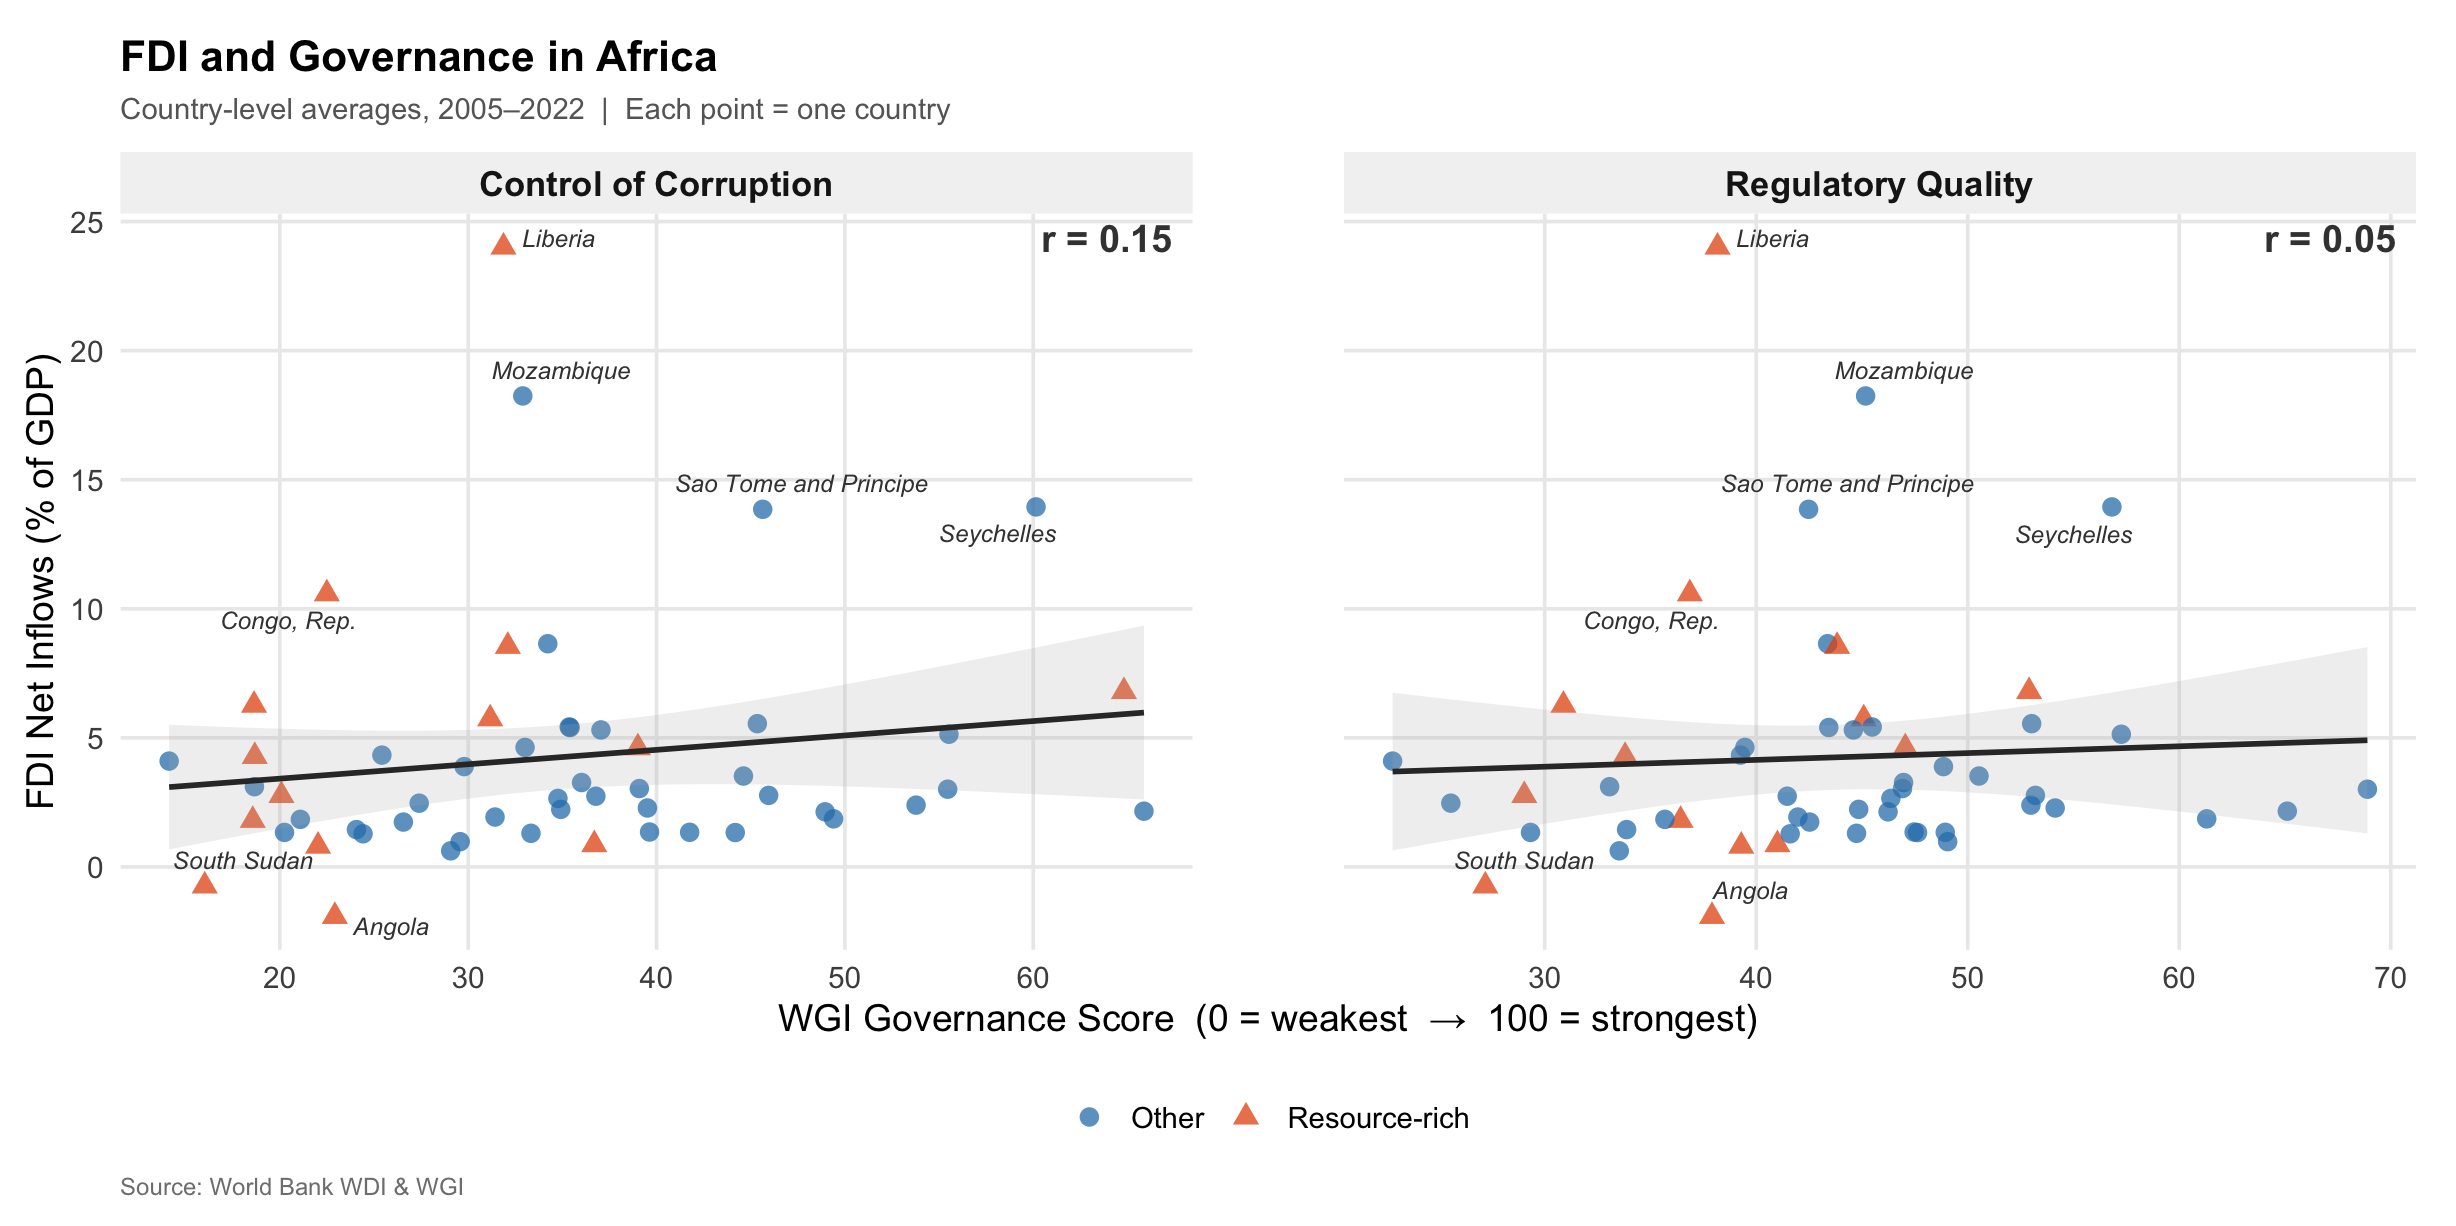
\includegraphics[keepaspectratio]{FDI_Governance.png}}

}

\caption{Figure 1: Scatter plots of country-level average FDI (\% of
GDP) against Control of Corruption (Panel A) and Regulatory Quality
(Panel B), 2005--2022. Resource-rich countries (top quartile of natural
resource rents) are shown as orange triangles. The weak positive
correlations suggest that neither governance dimension has a simple
unconditional relationship with FDI in Africa, motivating the
conditional interaction analysis below. Source: World Bank WDI \& WGI.}

\end{figure}%

The weak raw correlations in Figure 1 are consistent with neither
governance dimension having a simple unconditional relationship with FDI
across Africa. Resource-rich countries (orange triangles) are
distributed across the full range of governance scores, suggesting that
natural resource endowments do not systematically sort countries along
either dimension. This motivates the interaction specification:
governance may matter for FDI, but only under certain institutional
conditions.

Figure 2 offers a first look at the interaction by splitting the sample
at the median of regulatory quality (43.72).
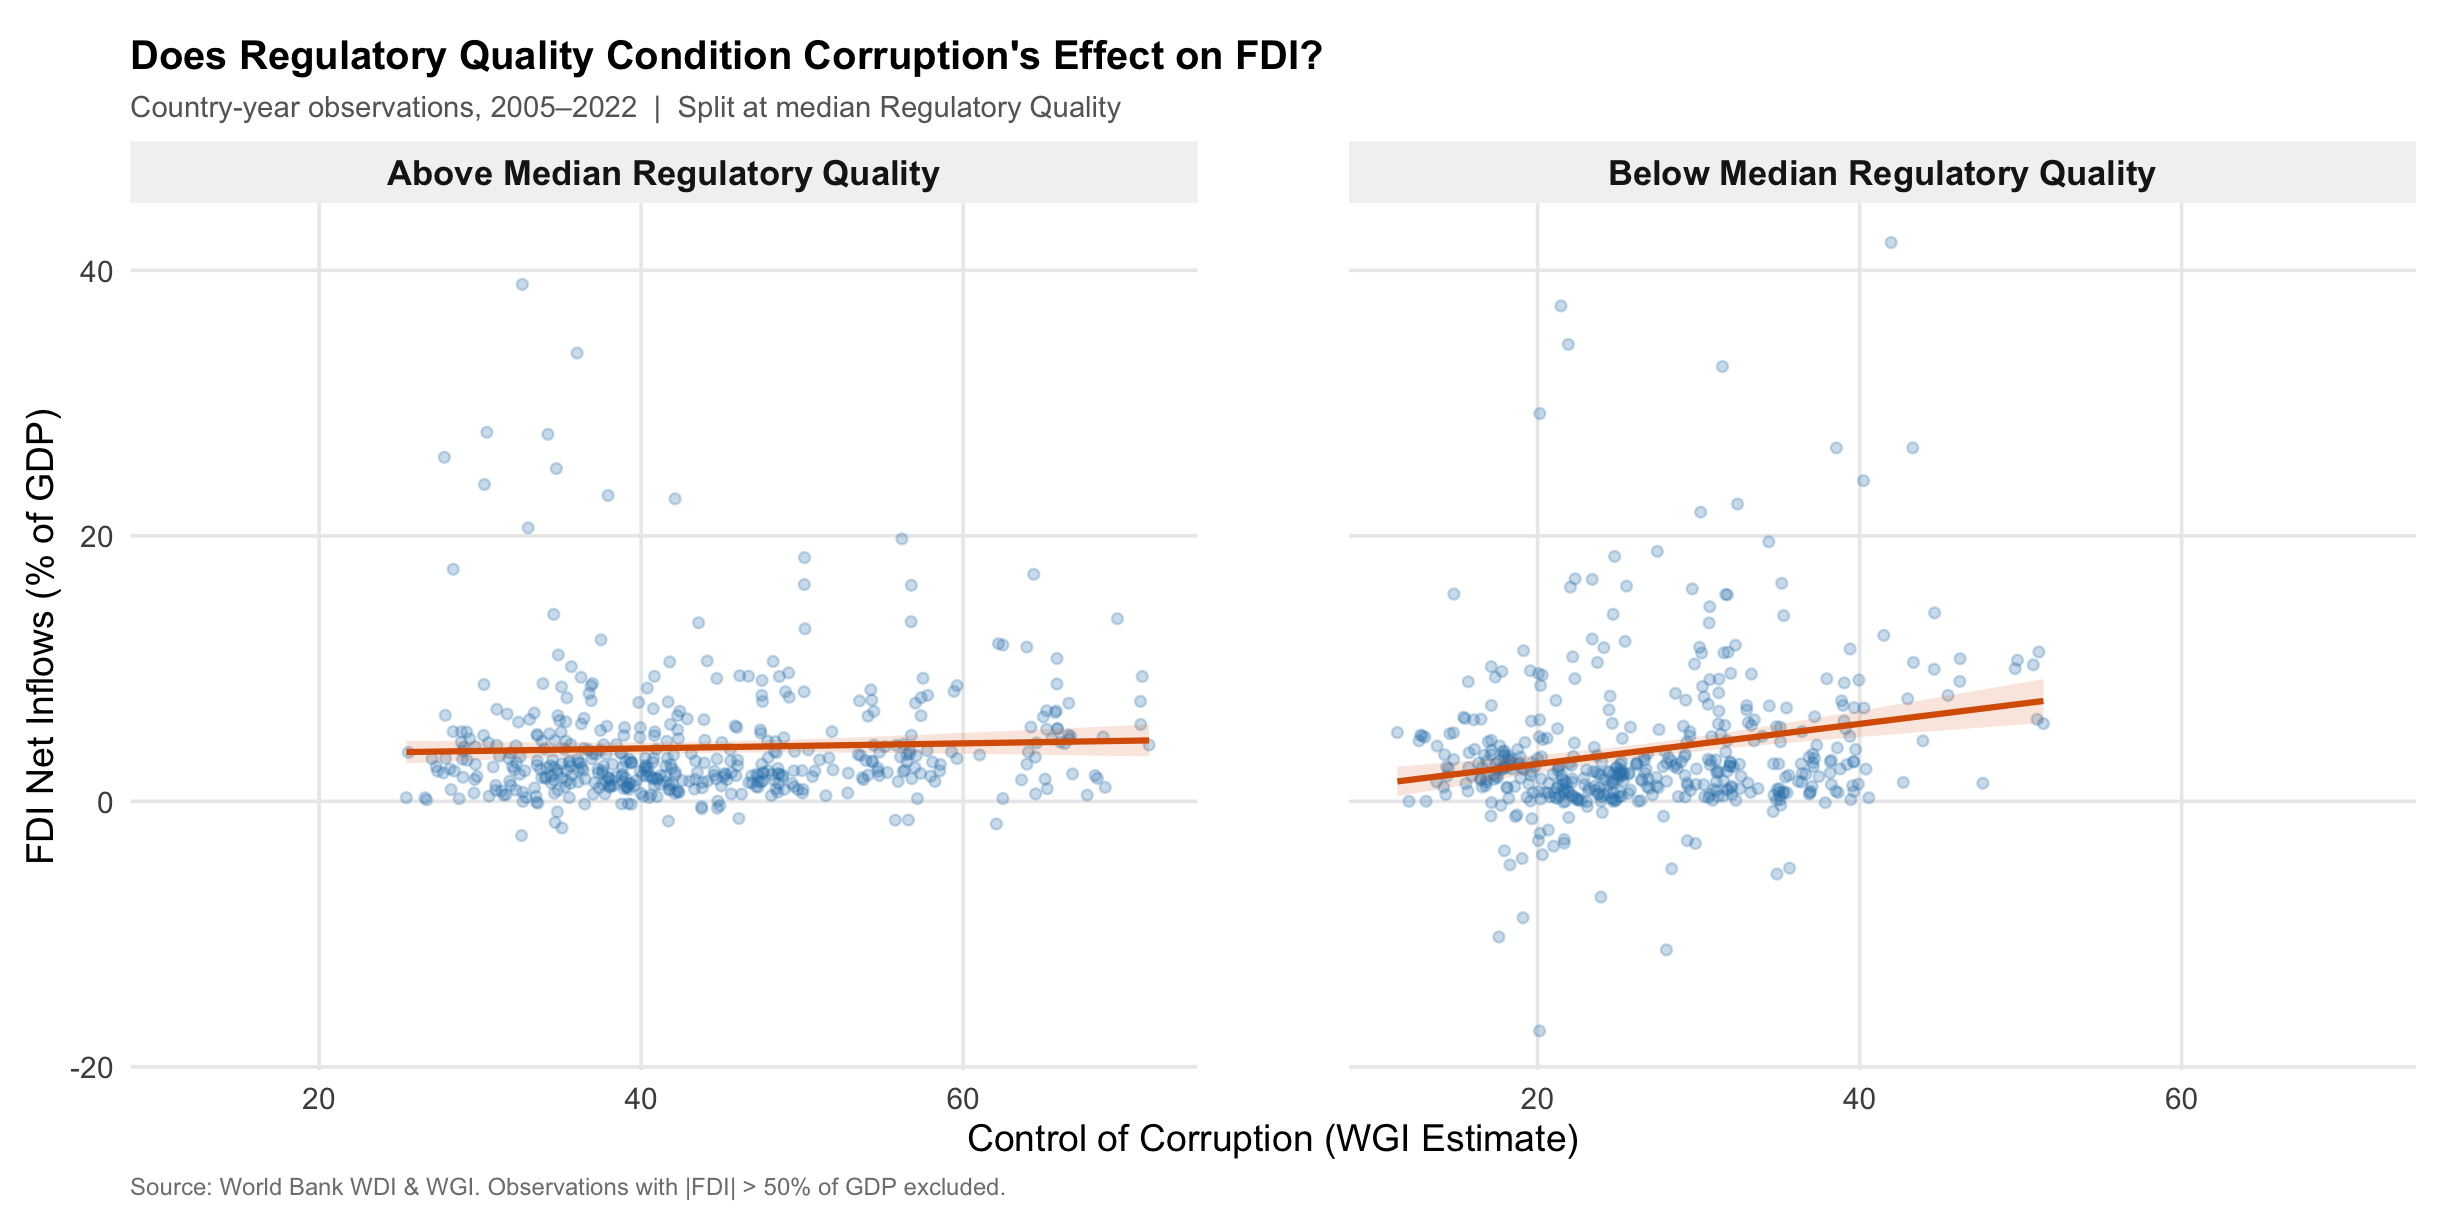
\includegraphics[width=1\linewidth,height=2\textheight]{CoC.png}

The split-sample pattern in Figure 2 is instructive. Among countries
with above-median regulatory quality, the relationship between
corruption control and FDI is essentially flat --- additional
anti-corruption gains appear to deliver little marginal investment
return where formal market institutions are already operative. Among
countries with below-median regulatory quality, by contrast, corruption
control is positively associated with FDI inflows, suggesting it
functions as a partial substitute for the regulatory infrastructure
those countries lack. This asymmetry constitutes preliminary visual
support for H1b (substitution) over H1a (complementarity), and motivates
the formal interaction test below.

The regression results are presented in Table 2, Column 1. The
interaction coefficient β\^{}3=−0.006\hat{\beta}\_3 = -0.006
β\^{}\hspace{0pt}3\hspace{0pt}=−0.006 (p\textless0.05p \textless{} 0.05
p\textless0.05) provides clear support for H1b (substitution), allowing
us to reject H1a (complementarity). To interpret this magnitude
concretely, consider two countries at the 25th and 75th percentiles of
Regulatory Quality --- approximately 37 and 51 on the 0--100 scale. At
the 25th percentile, a ten-point improvement in corruption control is
associated with a 1.0 percentage point increase in FDI as a share of GDP
(marginal effect ≈ 0.10). At the 75th percentile, the marginal effect is
approximately zero and may turn slightly negative --- consistent with
Figure 3, where the point estimate crosses the zero line around a
regulatory quality score of 48--50. Anti-corruption gains therefore
deliver substantially smaller, and eventually negligible, investment
returns in already well-regulated environments, a difference that is
economically meaningful given that the sample mean FDI share is just
4.35\% of GDP.

\begin{longtable}[]{@{}
  >{\raggedright\arraybackslash}p{(\linewidth - 8\tabcolsep) * \real{0.2000}}
  >{\centering\arraybackslash}p{(\linewidth - 8\tabcolsep) * \real{0.2000}}
  >{\centering\arraybackslash}p{(\linewidth - 8\tabcolsep) * \real{0.2000}}
  >{\centering\arraybackslash}p{(\linewidth - 8\tabcolsep) * \real{0.2000}}
  >{\centering\arraybackslash}p{(\linewidth - 8\tabcolsep) * \real{0.2000}}@{}}
\caption{Main Model and Placebo
Tests}\label{tbl-regression}\tabularnewline
\toprule\noalign{}
\begin{minipage}[b]{\linewidth}\raggedright
\end{minipage} & \begin{minipage}[b]{\linewidth}\centering
Main Model
\end{minipage} & \begin{minipage}[b]{\linewidth}\centering
Placebo: Voice
\end{minipage} & \begin{minipage}[b]{\linewidth}\centering
Placebo: Lagged
\end{minipage} & \begin{minipage}[b]{\linewidth}\centering
Placebo: Portfolio
\end{minipage} \\
\midrule\noalign{}
\endfirsthead
\toprule\noalign{}
\begin{minipage}[b]{\linewidth}\raggedright
\end{minipage} & \begin{minipage}[b]{\linewidth}\centering
Main Model
\end{minipage} & \begin{minipage}[b]{\linewidth}\centering
Placebo: Voice
\end{minipage} & \begin{minipage}[b]{\linewidth}\centering
Placebo: Lagged
\end{minipage} & \begin{minipage}[b]{\linewidth}\centering
Placebo: Portfolio
\end{minipage} \\
\midrule\noalign{}
\endhead
\bottomrule\noalign{}
\endlastfoot
Control of Corruption & 0.323* & 0.217 & & 0.071 \\
& (0.167) & (0.157) & & (0.200) \\
Control of Corruption (t−1) & & & 0.493** & \\
& & & (0.194) & \\
Regulatory Quality & 0.364* & & & 0.111 \\
& (0.184) & & & (0.217) \\
Regulatory Quality (t−1) & & & 0.368** & \\
& & & (0.178) & \\
Voice \& Accountability & & 0.007 & & \\
& & (0.130) & & \\
Corruption × Reg Quality & −0.006** & & & −0.002 \\
& (0.003) & & & (0.004) \\
Corruption × Voice \& Acct & & −0.003 & & \\
& & (0.003) & & \\
Corruption (t−1) × Reg Quality (t−1) & & & −0.009** & \\
& & & (0.004) & \\
Resource Rents (\% GDP) & −0.084* & −0.087** & −0.092** & −0.055 \\
& (0.043) & (0.043) & (0.044) & (0.079) \\
Trade (\% GDP) & 0.105*** & 0.102*** & 0.110*** & −0.017 \\
& (0.031) & (0.031) & (0.031) & (0.011) \\
Political Stability & −0.039 & −0.014 & −0.021 & −0.049 \\
& (0.040) & (0.035) & (0.040) & (0.048) \\
GDP per Capita & −0.000*** & −0.000*** & −0.000*** & −0.000 \\
& (0.000) & (0.000) & (0.000) & (0.000) \\
Num. Obs. & 774 & 774 & 731 & 431 \\
R² & 0.497 & 0.495 & 0.516 & 0.225 \\
R² Adj. & 0.445 & 0.443 & 0.463 & 0.107 \\
FE: country & ✓ & ✓ & ✓ & ✓ \\
FE: year & ✓ & ✓ & ✓ & ✓ \\
\end{longtable}

* p \textless{} 0.1, ** p \textless{} 0.05, *** p \textless{} 0.01.
Standard errors clustered by country in parentheses. Columns 1--3 use
FDI (\% GDP) as outcome; Column 4 uses portfolio equity (\% GDP). To
understand precisely where in the regulatory quality distribution the
moderation effect is statistically operative, Figure 3 plots the
marginal effect of corruption control on FDI across the full observed
range of regulatory quality with 95\% confidence intervals.

\begin{figure}[H]

{\centering 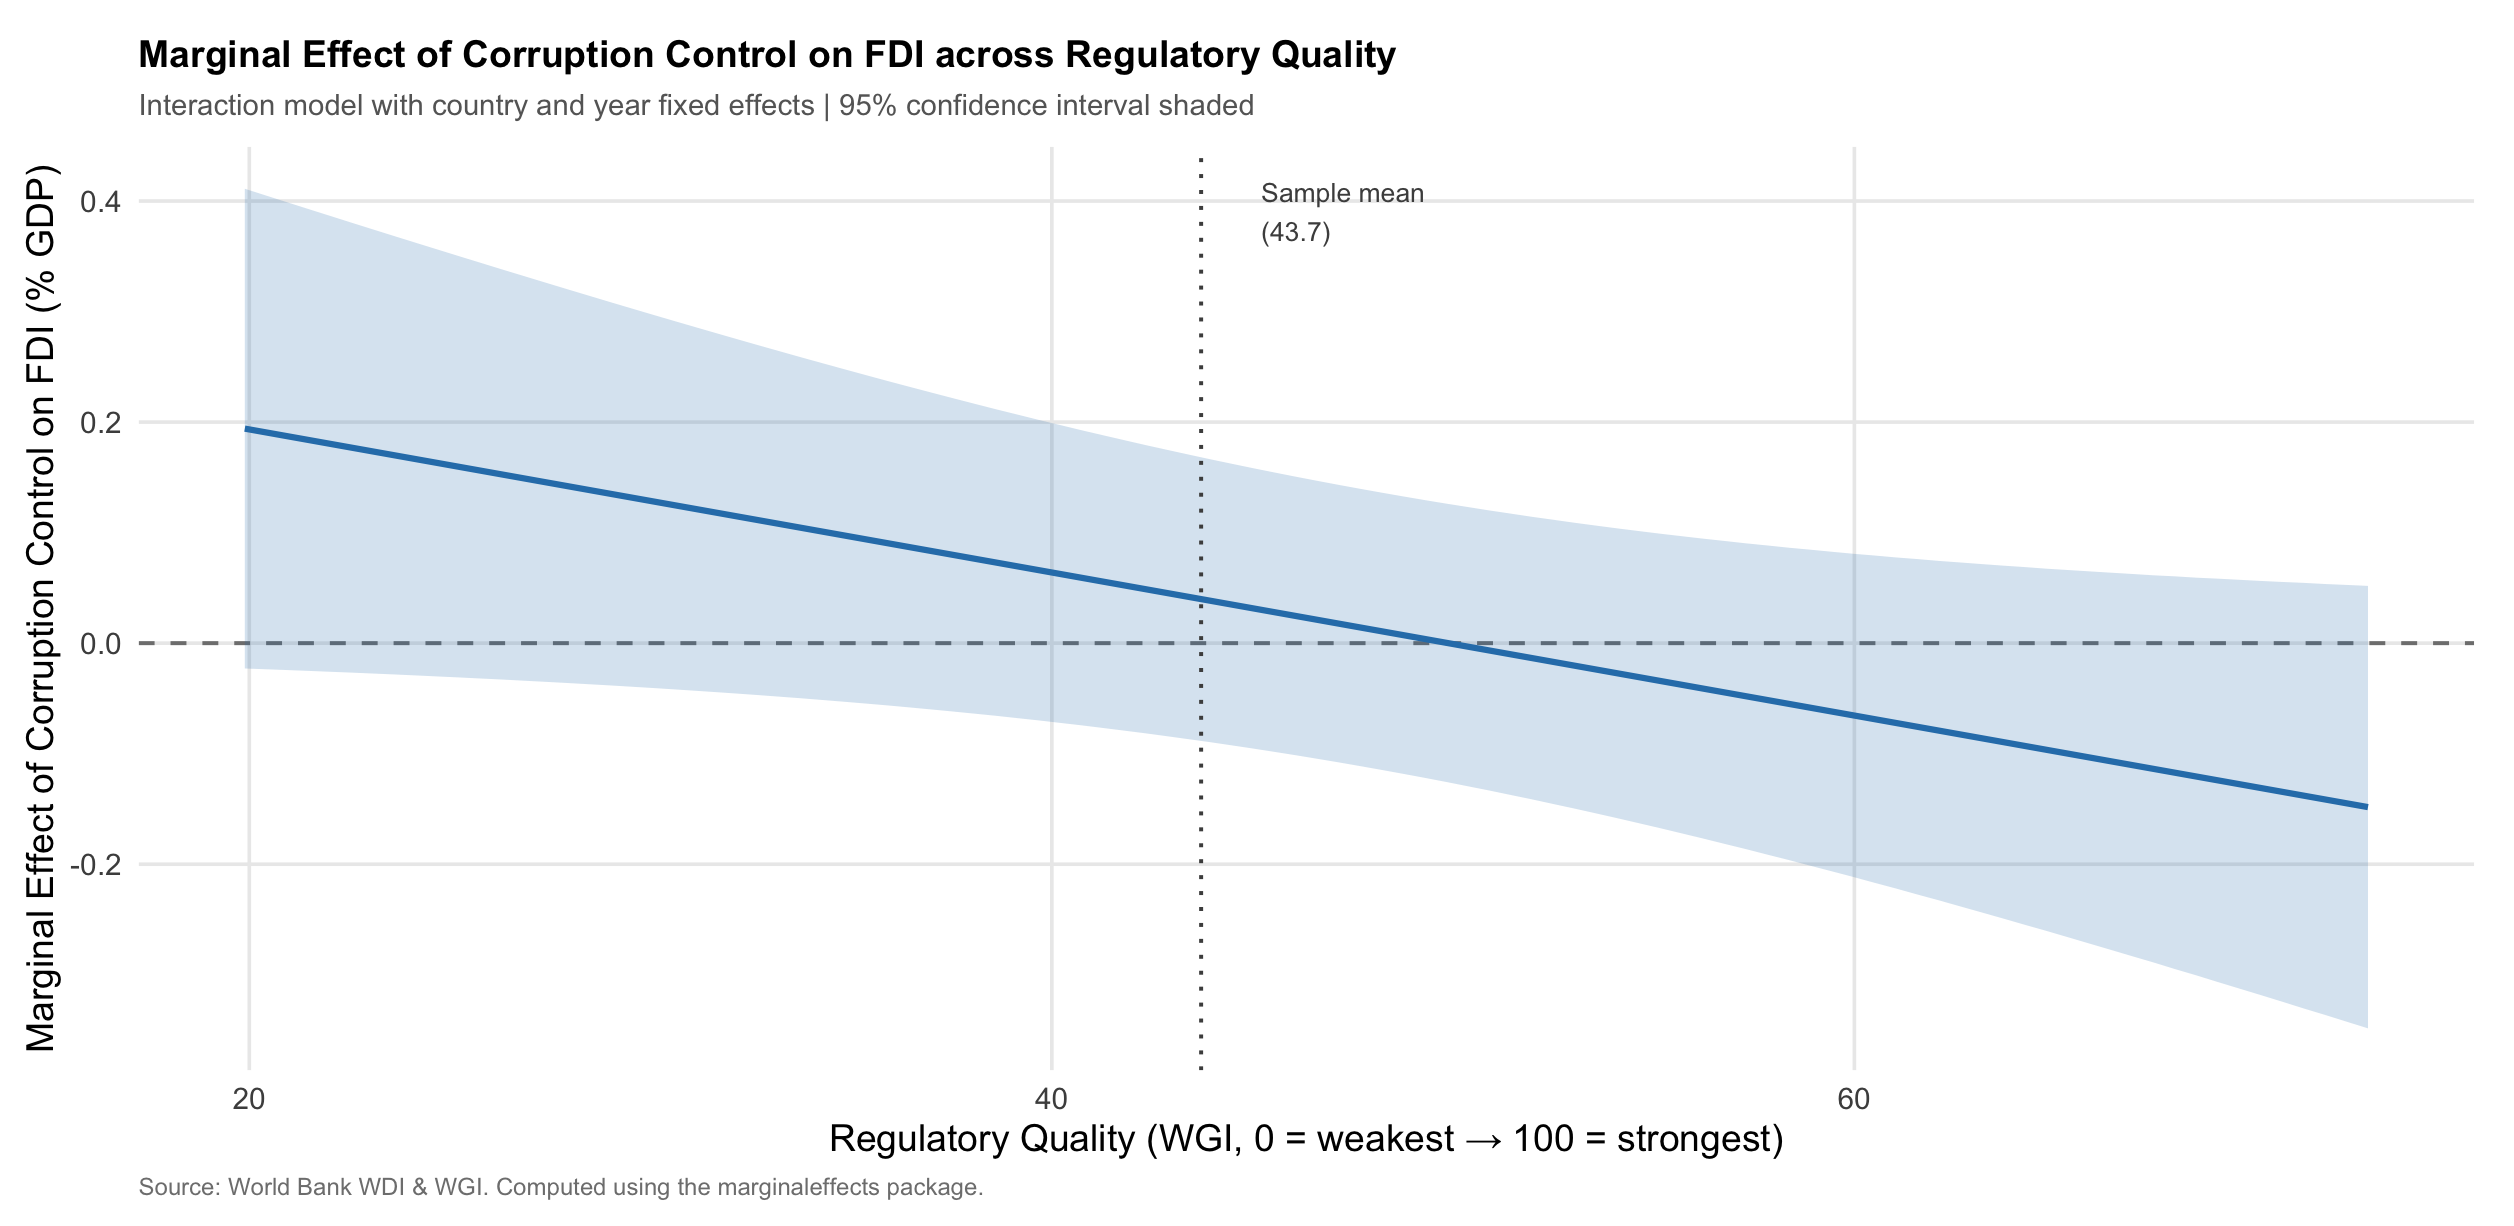
\includegraphics[width=1\linewidth,height=\textheight,keepaspectratio]{Marginal_Effect.png}

}

\caption{Figure 3: Marginal effect of corruption control (WGI) on FDI
net inflows (\% of GDP) across the observed range of Regulatory Quality,
estimated from the two-way fixed effects interaction model.}

\end{figure}%

Figure 3 reveals important heterogeneity in where the substitution
effect is statistically and substantively operative. At low levels of
regulatory quality (around 20 on the WGI scale), the marginal effect of
corruption control is positive --- approximately 0.20 percentage points
of FDI per GDP per unit improvement --- but is estimated with
considerable imprecision, with confidence intervals spanning zero. In
institutionally weak environments, corruption control neither reliably
attracts nor deters FDI, likely because the entire formal investment
framework is sufficiently underdeveloped that marginal anti-corruption
signals are insufficient to shift investor behaviour. As regulatory
quality rises toward and above the sample mean (43.7), the point
estimate declines monotonically, crossing zero around a score of 48--50
and turning statistically significant and negative at higher values,
where the confidence band lies entirely below the zero line. It is
precisely in Africa's better-governed economies --- where investors are
already operating through formal channels --- that further
anti-corruption progress is associated with reduced FDI inflows,
plausibly because stricter enforcement removes informal flexibility
without yet providing commensurate new formal assurances. Crucially,
given that WGI indices are perception-based and therefore subject to
classical measurement error, these estimates are likely attenuated
toward zero, suggesting that the true substitution effect at high
regulatory quality may be larger in magnitude than reported here.

\section{Empirical Extension}\label{empirical-extension}

The main finding --- that corruption control's association with FDI
diminishes and eventually turns negative as regulatory quality improves
--- could reflect two alternative explanations that must be ruled out
before the substitution interpretation can be sustained. First, the
negative interaction might be a generic ``good governance'' effect, in
which any pairing of institutional dimensions produces a similar
moderating pattern simply because governance indices are correlated with
one another. Second, the effect might be an artefact of the FDI measure
itself: long-horizon foreign direct investment requires firms to
physically embed in a host economy, navigating permits, contracts, and
local workforces, and so may be uniquely sensitive to the
regulatory--corruption nexus in ways that short-horizon financial flows
are not.

\textbf{Placebo 1: Non-market governance (Voice and Accountability).}
Column 2 replaces Regulatory Quality with the WGI Voice and
Accountability index, which captures political freedoms, civil
liberties, and press freedom. Critically, this dimension has no direct
bearing on permit issuance, contract enforcement, or market entry ---
the precise channels through which the substitution mechanism operates.
The flat slope in Figure 2's above-median panel, and the zero-crossing
in Figure 3, both implicate \emph{market-operational} institutions
specifically: environments where formal rules govern the day-to-day
transaction costs of doing business. Voice and Accountability does not
govern these transactions. If the Figure 3 pattern were simply a
reflection of correlated governance indices rather than a specific
institutional mechanism, the interaction with Voice and Accountability
should be similarly signed and significant. It is not: the coefficient
is −0.003 and statistically insignificant (p\textgreater0.1),
approximately half the magnitude of the main interaction and
indistinguishable from zero. This rules out a generic governance halo
interpretation and anchors the finding to the market-operational
channel.

\textbf{Placebo 2: Portfolio equity flows.} Column 4 replaces the
dependent variable with portfolio equity inflows (\% of GDP). Unlike
FDI, portfolio investment involves the acquisition of listed financial
assets rather than operational assets; portfolio investors do not build
facilities, hire local management, or repeatedly engage with regulatory
agencies. They are therefore largely insulated from the informal
flexibility that the substitution mechanism posits: the progressive
removal of that flexibility as regulatory quality improves --- visible
in Figure 3's declining marginal effect --- should not register in their
investment calculus. Consistent with this prediction, the interaction
coefficient for portfolio flows is -0.002 and statistically
insignificant, confirming that the pattern documented in Figures 2 and 3
is specific to investment modes that require sustained regulatory
engagement. Together, these tests triangulate the finding with
precision: the substitution effect identified in Figure 3 is specific to
a market-operational governance dimension rather than institutional
quality in general, and to long-horizon investment rather than financial
flows --- exactly the combination the proposed mechanism requires. The
placebo results also provide indirect reassurance that the correlated
structure of WGI indices is not mechanically generating the main result.

\textbf{Lagged specification.} Column 3 re-estimates the main model with
one-year lags on both governance variables. The sign, magnitude, and
significance of the interaction term are nearly identical to those in
Column 1, unsurprising given the high year-to-year persistence of WGI
scores, which change slowly by design. The lagged model therefore
largely reproduces the main result with a one-year offset rather than
providing genuinely independent evidence. It is retained for
completeness, but the two placebo tests, which vary the governance
dimension and the outcome variable rather than timing, are the more
informative robustness checks.

\section{Discussion and Policy
Implications}\label{discussion-and-policy-implications}

This analysis finds consistent support for the substitution mechanism
(H1b). In the African context, regulatory quality and corruption control
function as institutional substitutes: as formal market institutions
strengthen, the marginal investment return to anti-corruption progress
declines, eventually turning negative among the continent's
better-governed economies. Rather than resolving the ``grease the
wheels'' versus ``sand the wheels'' debate unconditionally, the results
suggest the answer is context-dependent --- corruption control sands the
wheels most where formal wheels already turn smoothly. The two-way fixed
effects design, lagged specification, and placebo tests collectively
make it difficult to attribute this pattern to generic governance
quality or short-horizon financial dynamics. Nevertheless, time-varying
omitted variables cannot be ruled out, and the WGI's perception-based
construction introduces classical measurement error that likely
attenuates estimates toward zero --- meaning the true substitution
effect is probably larger than reported here. Results should be read as
conservative conditional associations rather than clean causal
identification. The policy implications map directly onto the three
regimes visible in Figure 3. For weak-regulatory states such as Chad or
the Central African Republic, anti-corruption enforcement in isolation
will not move investors; the priority is foundational regulatory
infrastructure. For transition-zone economies around the sample mean,
such as Kenya, Senegal, Tanzania coordinated reform is warranted:
regulatory deepening and anti-corruption enforcement should advance
together so that firms exiting informal channels find functioning formal
alternatives. For better-governed economies such as Botswana, Mauritius,
or Rwanda, the finding carries a counterintuitive warning: aggressive
enforcement is associated with lower FDI, likely because investors lose
informal flexibility before formal assurances materialise. Sequencing
matters here, enforcement should be paired with explicit strengthening
of investor protections and regulatory predictability. Future research
should pursue cleaner identification through historical institutional
instruments or quasi-experimental shocks such as FATF grey-listing, and
firm-level data to trace the mechanism to individual investment
decisions.

\begin{center}\rule{0.5\linewidth}{0.5pt}\end{center}

\section*{References}\label{references}
\addcontentsline{toc}{section}{References}

\phantomsection\label{refs}
\begin{CSLReferences}{1}{0}
\bibitem[\citeproctext]{ref-benassy2007}
Bénassy-Quéré, Agnès, Maylis Coupet, and Thierry Mayer. 2007.
{``Institutional Determinants of Foreign Direct Investment.''} \emph{The
World Economy} 30 (5): 764--82.
\url{https://doi.org/10.1111/j.1467-9701.2007.01022.x}.

\bibitem[\citeproctext]{ref-lakha2024}
Lakha, Bhavna, Adeola Oyenubi, David Fadiran, and Nihaal Naik. 2024.
{``Governance and the Relationship Between Corruption and {FDI} in
{Africa}: A Threshold Regression Analysis.''} \emph{International Review
of Applied Economics} 38 (6): 613--32.
\url{https://doi.org/10.1080/02692171.2024.2382112}.

\bibitem[\citeproctext]{ref-mauro1995}
Mauro, Paolo. 1995. {``Corruption and Growth.''} \emph{The Quarterly
Journal of Economics} 110 (3): 681--712.
\url{https://doi.org/10.2307/2946696}.

\bibitem[\citeproctext]{ref-meon2005}
Méon, Pierre-Guillaume, and Khalid Sekkat. 2005. {``Does Corruption
Grease or Sand the Wheels of Growth?''} \emph{Public Choice} 122 (1--2):
69--97. \url{https://doi.org/10.1007/s11127-005-3988-0}.

\bibitem[\citeproctext]{ref-quazi2014}
Quazi, Rahim, Vijay Vemuri, and Mohamed Soliman. 2014. {``Impact of
Corruption on Foreign Direct Investment in {Africa}.''}
\emph{International Business Research} 7 (4): 1--10.
\url{https://doi.org/10.5539/ibr.v7n4p1}.

\bibitem[\citeproctext]{ref-unctad2026}
United Nations Conference on Trade and Development. 2026. {``Global
Investment Trends Monitor, No.~50: Global {FDI} up 14\% in 2025.''}
UNCTAD/DIAE/IA/INF/2026/1. UNCTAD.
\url{https://unctad.org/publication/global-investment-trends-monitor-no-50}.

\bibitem[\citeproctext]{ref-wei2000}
Wei, Shang-Jin. 2000. {``How Taxing Is Corruption on International
Investors?''} \emph{The Review of Economics and Statistics} 82 (1):
1--11. \url{https://doi.org/10.1162/003465300558533}.

\end{CSLReferences}




\end{document}
